\documentclass{article}

% set font encoding for PDFLaTeX or XeLaTeX
\usepackage{ifxetex}
\ifxetex
  \usepackage{fontspec}
\else
  \usepackage[T1]{fontenc}
  \usepackage[utf8]{inputenc}
  \usepackage{lmodern}
  \usepackage{graphicx}
\fi

% used in maketitle
\title{Características, limitaciones y bondades de Jupyter Notebook como entorno de programación}
\author{Mariana Ruíz Quintín}

% Enable SageTeX to run SageMath code right inside this LaTeX file.
% documentation: http://mirrors.ctan.org/macros/latex/contrib/sagetex/sagetexpackage.pdf
% \usepackage{sagetex}

\begin{document}
\maketitle

\section{Introduction}

Jupyter Notebook es una aplicación web que permite crear y compartir documentos que contienen código fuente, ecuaciones, visualizaciones y texto explicativo.  Generalmente esta herramienta es utilizada para el aprendizaje del lenguaje de programación python, la limpieza y transformación de datos científicos, la simulación numérica, el modelado estadístico y puede abarcar muchas otras áreas.

\subsection{Características}

Las características de esta herramienta son:

 - De fácil instalación gracias a estar presente en la Suite Anaconda Distribution.

- Posee una avanzada interfaz web que permite combinar código fuente, textos, formulas, figuras y multimedia en un solo documento.

- La integración de diverso tipos de información nos permite dar explicaciones más adecuada de nuestros programas o de los conceptos que estemos aprendiendo.

- Permite el acceso desde cualquier lugar sin necesidad de instalación de otros servicios, ya que funciona como cliente servidor. De igual manera, Se puede ejecutar en un escritorio local o en servidor remoto.

- Aunque el lenguaje de programación fundamental en Jupyter Notebook es Python, esta aplicación también es compatible con más de 40 lenguajes, entre los que destacan R, Julia y Scala.

- Permite el intercambio de documentos de Jupyter a través de servicios de terceros.
Podemos ejecutar y visualizar imágenes, videos, LaTeX y JavaScript, además de manipular los resultados de los mismos en tiempo real.

- Cuenta con un administrador de documentos avanzado, que permite visualizar los archivos compatible con Jupyter Notebook que esten alojados en nuestro equipo.

- Los documentos realizados en Jupyter Notebook se pueden exportar a diferentes formatos estáticos incluyendo HTML, reStructeredText, LaTeX, PDF y presentaciones de diapositivas.

- Es compatible con nbviewer el cual permite que portar nuestros documentos de Jupyter Notebook a la nube como una página web estática, la cuál podrá ser visualizada por cualquiera sin necesidad de instalar el Jupyter Notebook .

\subsection{Limitaciones}


Se necesitan conocimientos de programación para poder aprovecharlo de la mejor y mayor manera. Es decir, conocer y comprender el código con el que se pretende trabajar.

\subsection{Bondades}

Los beneficios con los que contamos al manejar esta herramienta son el poder utilizar texto, ecuaciones, imágenes, fórmulas, etcétera, esto en forma de código, siempre y cuando se tengan los conocimientos básicos de éstos o bien se dominen. Este es un beneficio ya que el resultado que arroja es limpio y estético, con estructuras de datos rápidas, flexibles y expresivas. Además de todo esto se tiene que se puede utilizar para manejar datos científicos al igual que se puede desarrollar en otras áreas.

Además de esto se tienen herramientas nuevas como el cambio e compatibilidades, mejoras de rendimiento, mejoras en manejo de errores durante asignación de elementos, cambios de documentación, entre muchos otros.

Algunos ejemplos de los resultados que se pueden obtener solo los siguientes, los cuales son resultado del manejo de datos del sistema meteorológico.


 \begin{figure}[ht!]
  \centering
   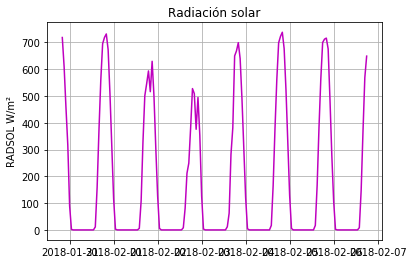
\includegraphics[width=0.8\linewidth]{Radiacionsolar.png}
  \end{figure}


 \begin{figure}[ht!]
   \centering
   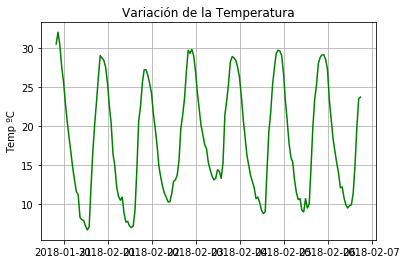
\includegraphics[width=0.8\linewidth]{Variaciondelatemperatura.png}
  \end{figure}


 \begin{figure}[ht!]
   \centering
   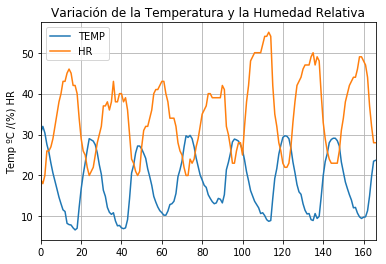
\includegraphics[width=0.8\linewidth]{Variaciondelatemperaturayhumedadrelativa.png}
  \end{figure}


\subsection{Bibliografía}

Desconocido. (2017, Diciembre). Pandas: Potente kit de herramientas de análisis de datos de Python. https://pandas.pydata.org/pandas-docs/stable/index.html

Lagarto. (2017, Septiembre). Jupyter notebook: documenta y ejecuta código desde el navegador. https://blog.desdelinux.net/jupyter-notebook/

%¿Cuál es tu primera impresión de Jupyter Notebook? Al principio me pareció un poco difícil ya que no comprendía bien que era lo que estaba haciendo.
%¿Se te dificultó leer código en Python? Si
%¿En base a tu experiencia de programación en Fortran, que te parece el entorno de trabajar en Python? Me gusta más, es más fácil.
%A diferencia de Fortran, ahora se producen las gráficas utilizando la biblioteca Matplotlib. ¿Cómo fue tu experiencia?. Me gustan más los resultados obtenidos, solo sería cuestión de práctica para saber que tanto puedo hacer.
%En general, ¿qué te pereció el entorno de trabajo en Python? Me pareció más cómodo ya que al tener algún error me pareció muy bien que no fue laborioso corregirlo.
%¿Qué opinas de la actividad? ¿Estuvo compleja? ¿Mucho material nuevo? ¿Que le faltó o que le sobró? ¿Qué modificarías para mejorar? Estvo bien la actividad. Y si mucho material nuevo par mí, ya que no se me da muy bien programar.
%¿Comentarios adicionales que desees compartir? Ninguna.

\end{document}

